\section{Método}

\subsection{Implementación}

Se construyó un prototipo de \eyetracker web formado por módulos preexistentes
y desarrollos propios.
El contexto remoto no supervisado explicado previamente tiene implicaciones
sobre su implementación.
Este debe funcionar en un navegador web, y en particular debe ser compatible
con la herramienta de experimentos conductuales \jspsych. 
l sujeto no contará con alguien que lo supervise durante el experimento ni con
una estructura que le ayude a mantener la cabeza quieta.
Por lo tanto se deberá definir algún criterio que nos indique cuándo es
necesaria una recalibración.

Se implementó entonces una herramienta que provee una estimación de la mirada
con fases explícitas de calibración, verificando a lo largo del tiempo si el
sujeto movía la cabeza respecto de su posición durante la calibración.
De \webgazer se reutilizó principalmente su modelo de estimación de la mirada y
utilidades como aquella que muestra en la pantalla la coordenada estimada de la
mirada.
Sin embargo, se descartó utilizar sus elementos de calibración pues no aplican
a nuestro caso.
Además, se mantuvo una división explícita entre el código correspondiente al
\eyetracking (el \textit{core}) respecto de la interfaz con \jspsych.
Al prototipo implementado se le dio el nombre \rastoc para poder referirse a él
dentro del código.

\begin{figure}
    \centering
    \includegraphics[width=0.8\linewidth]{media/components.png}
    \caption{Relaciones entres componentes implementados y componentes
    existentes}
    \label{fig:components}
\end{figure}

\subsubsection{Calibración}

La calibración del sistema consiste en acumular un conjunto de pares
$<$\textit{features} de los ojos, coordenada$>$.
Cada uno de estos pares representa a qué coordenada de la pantalla estaba
mirando el sujeto cuando la imagen de sus ojos tenía un determinado aspecto.
Las \textit{features} utilizadas incluyen las coordenadas y dimensiones del
recuadro capturado en relación al \textit{frame} entero, así como un vector
correspondiente al recuadro en sí como una imagen.
La conversión de \textit{frames} a \textit{features} es realizada continuamente
por \webgazer (cf. estimación de la mirada).

La construcción del conjunto de calibración se hará en base a una secuencia de
interacciones por parte del sujeto.
Al momento de tal interacción se guardará el par formado por el último
\textit{frame} capturado y la coordenada de la interacción.
Esto puede hacerse únicamente luego de iniciar una fase explícita de
calibración.
La Figura \ref{fig:calibration_cycle} ilustra las distintas etapas de
calibración recorridas por el sistema.
Al finalizar esta etapa el conjunto acumulado se utiliza para: a) entrenar el
modelo de regresión utilizado por \webgazer para estimar la mirada; b)
instanciar el mecanismo de detección de movimiento.

\begin{figure}
    \centering
    \includegraphics[width=0.8\linewidth]{media/calibration_cycle.png}
    \caption{Posibles estados de calibración del prototipo implementado}
    En los estados con linea punteada el sistema no podrá realizar estimaciones
    de la mirada.
    Notar que se continuará dando estimaciones incluso cuando se considere que
    el sistema se ha descalibrado.
    Los distintos mecanismos de calibración se adaptan a este esquema y
    difieren en cómo el usuario realiza el mapeo coordenada a \textit{frame}.
    \label{fig:calibration_cycle}
\end{figure}

Al iniciar una fase explícita de calibración, el \textit{core} provee dos
métodos para indicar tales coordenadas.
El primero (\texttt{calibrationType === “click”}) permite al experimentador
indicar que cada click realizado en la pantalla tendrá que ser usado para
calibrar el sistema.
El segundo (\texttt{calibrationType === “external”}) devuelve un
\textit{callback} que el experimentador podrá utilizar cuando lo desee,
permitiéndole entonces implementar el mecanismo de calibración que prefiera.
Se asume siempre que el sujeto estará mirando a la coordenada input.

A nivel \jspsych, a través de estos dos mecanismos se ofrecen dos opciones
distintas que el experimentador puede utilizar para que el sujeto calibre el
sistema.
Por un lado, está la calibración libre, en la cual el sujeto tendrá que
clickear en la pantalla mientras mira el puntero.
Por otro lado está la calibración asistida, que funciona a través del paquete
\psychophysics [0.2] y durante la cual se dibujan una serie de estímulos en la
pantalla, ilustrado en la Figura \ref{fig:calibration_stimulus}.
Cada vez que aparece uno de estos, el sujeto tendrá que fijar la mirada en él y
presionar la barra de espacio para indicar que lo está mirando.
Buscando minimizar la cantidad de puntos mostrados, esta calibración prioriza
asegurar buenas estimaciones únicamente en las regiones de interés, que en el
caso de la tarea de antisacadas son tres.
Para esto se eligen mostrar estímulos de calibración sobre un eje horizontal
central en el centro, en la derecha y en la izquierda.

\begin{figure}
    \centering
    \includegraphics[width=0.4\linewidth]{media/calibration-stimulus-left.png}
    \includegraphics[width=0.4\linewidth]{media/calibration-stimulus-center.png}
    \includegraphics[width=0.4\linewidth]{media/calibration-stimulus-right.png}
    \caption{Estímulos de calibración}
    Al realizar una calibración asistida el sujeto es presentado con estímulos
    visuales en las regiones de interés.
    Para avanzar con la calibración, el sujeto deberá fijar la mirada en cada
    estímulo que aparece y luego presionar la barra de espacio.
    \label{fig:calibration_stimulus}
\end{figure}

Finalizada la etapa explícita de calibración, el sistema puede recalibrarse
cuando se considere necesario.
Para esto debe iniciarse una nueva fase de calibración explícita que
reemplazará los datos de la calibración anterior.

\subsubsection{Validación}

La interfaz \jspsych provee la opción de realizar una validación luego de cada
calibración.
En esta se muestran progresivamente estímulos en el centro y en las cuatro
esquinas de la pantalla.
Al igual que con la calibración asistida, cada vez que aparezca un estímulo, el
sujeto deberá fijar la mirada en él y presionar la barra de espacio.
Durante la presentación de estos estímulos se estará estimando la mirada en la
pantalla.
Idealmente se verificaría que durante un período previo a la interacción del
sujeto estas estimaciones coincidan en algún grado con las coordenadas de los
estímulos presentados \cite{huang_2016_pace}.
Sin embargo, debido a las desviaciones detectadas en la primer fase de
experimentación (cf. sección \ref{section:skewed-estimates}) se
verifica, en cambio, un correcto posicionamiento relativo.
Dicho de otra manera, en lugar de verificar que al mostrar un estímulo en la
esquina superior derecha las estimaciones coinciden con la coordenada de tal
estímulo, se verificará en cambio que tales estimaciones están a la derecha de
las estimaciones obtenidas al mostrar el estímulo superior izquierdo.
Debido a lo ya mencionado respecto de los mecanismos de calibración (cf.
sección \ref{section:intro:calibration}) y a que en este trabajo no interesa
analizar las coordenadas verticales de las estimaciones (pues implementamos
únicamente la tarea de antisacada) se optó además por verificar únicamente que
hubiera un correcto posicionamiento relativo horizontal.
Queda pendiente estudiar e implementar mecanismos de calibración y validación
que balanceen correctamente experiencia de uso y calidad de las estimaciones.

Como se detallará en la sección de preprocesamiento (sección
\ref{section:preprocessing}), este mecanismo de validación facilita luego la
implementación de una rutina de normalización.

\subsubsection{Estimación de la mirada}

Se delegó la estimación de la mirada al paquete \webgazer
\cite{papoutsaki_2016_webgazer}.
Esta se basa en un modelado explícito de la cara para localizar los ojos y un
modelo por apariencia para estimar la mirada.

La localización de los ojos se realiza a través del modelo de \textit{facemesh}
de \texttt{TensorFlowJS}
\footnote{\url{https://github.com/tensorflow/tfjs-models/tree/master/face-landmarks-detection}}.
Utilizando los \textit{keypoints} obtenidos se recorta de cada \textit{frame}
un recuadro para cada ojo.
No está claro si este mecanismo es ideal pues, por ejemplo, se está modelando
toda la cara mientras que nos importa únicamente la posición de un par de
recuadros de los ojos.
No sólo parece excesivo en términos de costos computacionales, si no que al no
estar modelando específicamente los ojos sería esperable no obtener la mejor
precisión que podría obtenerse.
Existen en cambio mecanismos específicos para la localización de los ojos
[10.1].

Cada recuadro tiene luego su tamaño ajustado a una dimensión fija de 10x6
píxeles.
Se los convierte luego a una escala de grises y son ecualizados a través de
histogramas.
De esta manera, para cada \textit{frame} de la webcam se obtiene un vector de
120 dimensiones correspondiente a la apariencia de los dos ojos.
De este universo 120D se pasa luego al universo de coordenadas 2D a través de
un modelo de \textit{ridge regression}.
Los coeficientes de este modelo se calculan al finalizar la fase explícita de
calibración.

\subsubsection{Descalibración}

En nuestro contexto web es inevitable una eventual descalibración del sistema,
es decir alcanzar un estado del sistema tal que las estimaciones arrojadas no
tienen suficiente calidad.
Entonces, debe proveerse algún mecanismo que identifique tal situación para
poder a su vez informar cuándo es necesaria una recalibración.

A modo de primer acercamiento se implementó un mecanismo basado en detectar
movimiento de la cabeza del sujeto.
En base al conjunto de \textit{features} de ojos capturados al calibrar, se
obtienen un par de conjuntos de rectángulos que contienen a los ojos en cada
uno de los correspondientes \textit{frames}.

Se definen luego, para cada ojo, un multipoligono (i.e., una forma geométrica
definida en base a múltiples polígonos) correspondiente a la unión de los
rectángulos de cada ojo, agrandados luego por un factor de 1.8 (elección
arbitraria basada en experimentación al desarrollar el prototipo).
El multipoligono obtenido para cada ojo representa el espacio dentro del cual
el recuadro del ojo deberá mantenerse para que se considere que no hubo
movimiento significativo.
Si a partir de algún \textit{frame} el recuadro de alguno de los ojos sale de
su multipoligono se considerará al sistema como descalibrado.

TODO: El párrafo que viene me parece que se repite con lo que quedó en la
conclu

El mecanismo propuesto es únicamente un primer acercamiento al problema de
detectar la descalibración del sistema.
En contextos de laboratorio es posible implementar modelos de estimación de la
mirada invariantes a movimientos de cabeza [10.1].
Además, al estar el movimiento de la cabeza habitualmente restringido, la
detección de descalibración suele ser menos relevante que en el contexto web
remoto.
Sin embargo, los \eyetrackers comerciales implementan mecanismos consistentes
en mostrar regularmente un punto en la pantalla para detectar si la estimación
de la mirada coincide con la coordenada del estímulo (e.g., \textit{drift
correction} en el \eyetracker \textit{EyeLink}).
Este mecanismo u otros podrían implementarse para asistir o reemplazar al
mecanismo implementado actualmente.

\subsubsection{Playgrounds}

Para ambas interfaces implementadas se construyó también un \textit{playground}
que permitiera interactuar con ellas.
El del \textit{core} (Figura \ref{fig:rastoc-playground}) permite realizar
calibraciones libres y visualizar la coordenada estimada de la mirada en la
pantalla al mismo tiempo que imprime ciertos datos de la calibración.
El de \jspsych (Figura \ref{fig:rastoc-jspsych-playground}) implementa un
\textit{timeline} de la misma librería.
El objetivo de ambos fue facilitar el desarrollo del prototipo.

\begin{figure}
    \centering
    \frame{\includegraphics[width=0.8\linewidth]{media/rastoc-jspsych-playground-presentation.png}}
    \caption{\texttt{rastoc-jspsych}’s playground}
    Las distintas utilidades de la interfaz \jspsych son provistas, permitiendo
    ciclar sobre ellas.
    Se puede elegir entre:
    a) calibrar libremente;
    b) calibrar asistidamente;
    c) mostrar un HTML básico mientras se estima la mirada;
    d) realizar una secuencia de repeticiones de una tarea de juguete mientras
    entre repeticiones se asegura la correcta calibración del sistema;
    e) finalizar la sesión para exportar la data recolectada.
    \label{fig:rastoc-jspsych-playground}
\end{figure}

\begin{figure}
    \centering
    \frame{\includegraphics[width=0.8\linewidth]{media/rastoc-playground-presentation.png}}
    \caption{\texttt{rastoc}’s playground}
    Información del estado del \eyetracker es presentada al mismo tiempo que se
    permite realizar calibraciones libres.
    El recuadro verde corresponde a la posición dentro de la cual el paquete
    \webgazer exige que aparezca la cabeza, los rectángulos rojos corresponden
    a los recuadros de los ojos en cada \textit{frame} y los rectángulos azules
    corresponden a las posiciones dentro de las cuales los recuadros de los
    ojos deben mantenerse para considerar que no hubo movimiento.
    \label{fig:rastoc-playground}
\end{figure}

\subsubsection{Detección de sacadas}

En la primera instancia se detectaron las sacadas buscando únicamente cuándo
las estimaciones post normalización cruzaban los umbrales 0.6 o -0.6 unidades
(post normalización al rango [-1, 1]) para respectivamente detectar sacadas
hacia el estímulo visual o en dirección contraria a él.

Para la segunda instancia se consideró como sacadas a los intervalos cuya
duración fuera mayor a 40 ms, tuvieran estimaciones monótonas crecientes o
decrecientes, hubieran recorrido al menos 0.6 unidades (post normalización al
rango [-1, 1] según los estímulos de validación) y tuvieran una velocidad
promedio de al menos 0.15 unidades / 100 ms.
Pueden realizarse mejoras en este punto, aunque tendrá que considerarse las
limitaciones propias del contexto (e.g., frecuencia de muestreo del orden de
los 25 Hz en contraposición a los 300 Hz reportados en herramientas
profesionales).


\subsection{Modificaciones a WebGazer}

En fases iniciales del desarrollo descripto en la sección previa se encontró
una falla vital en el paquete \webgazer.
Tal falla hacía que el paquete dejara de funcionar.
Si bien no ocurría en cualquier computadora, podía suceder en tiempos menores a
diez minutos (limitando el experimento).
Este problema había sido reportado ya en octubre del 2020
\footnote{\url{https://github.com/brownhci/WebGazer/issues/171}} sin mucha
respuesta, por lo que se lo reportó también a la comunidad de \jspsych
\footnote{\url{https://github.com/jspsych/jsPsych/discussions/2490}}.
Para nuestro caso de uso son esperables experimentos con duraciones cercanas a
los 20 minutos, por lo que dificultaba el uso de \webgazer en nuestra
implementación.
Se decidió investigar y modificar el paquete con el objetivo de corregir la
falla en cuestión.
Se realizaron las siguientes modificaciones, la última siendo aquella que
resolvió el problema:
\begin{enumerate}
    \item
    Reutilización del \textit{facemesh} interno de \webgazer\footnote{diff:
    \url{https://github.com/ffigari/WebGazer/commit/7c6b7fb4dcefea2b85d7a24b3e86bd9a31b938d4}}:
    Al implementar el mecanismo de detección de movimiento se agregó un modelo
    de \textit{facemesh} propio externo al paquete \webgazer.
    Ante la hipótesis de que esto estuviera causando una sobrecarga de
    recursos, se eliminó este \textit{facemesh} externo y se expuso en cambio
    el modelo interno.
    Para lograr esto, a medida que se calculan las \textit{features} de los
    ojos en cada \textit{frame}, se agregó la emisión de eventos
    \textit{custom} de \js que notificaban constantemente las actualizaciones
    permitiendo así su propagación.
    \item
    Se evitaron recomputaciones innecesarias de coeficientes\footnote{diff:
    \url{https://github.com/ffigari/WebGazer/commit/16f69474d40132c7faa826b2afc7fd464bc6c6c5}}:
    \webgazer está diseñado para permitir un agregado constante de datos de
    calibración en base a movimientos del puntero.
    Los coeficientes del modelo deben recalcularse cada vez que se modifique el
    conjunto de calibración.
    En la implementación original los coeficientes del modelo de regresión se
    recomputan en cada \textit{frame}, probablemente debido a que el agregado
    mencionado puede ocurrir en cualquier momento.
    Por otro lado, en nuestro caso de uso se agregará data de calibración
    únicamente durante la fase explícita de calibración.
    Alcanza entonces computar los coeficientes del modelo de regresión
    únicamente al finalizar la fase explícita de calibración.
    Se modificó entonces el paquete y su interfaz para permitir tal
    comportamiento.
    Al igual que la mejora anterior, esto no resolvió la falla pero sí reduce
    la carga sobre los recursos y resulta en una implementación más coherente
    al diseño que se busca implementar.
    \item
    Actualización del modelo interno de \textit{facemesh}\footnote{diff:
    \url{https://github.com/ffigari/WebGazer/commit/e5df9f9c3521ec3e384e962db49d94b2411789bb}}:
    Originalmente \webgazer utilizaba el paquete
    \texttt{@tensorflow-models/facemesh}\footnote{\url{https://www.npmjs.com/package/@tensorflow-models/facemesh}}
    para generar el modelo de \textit{facemesh}.
    Tal paquete se encuentra sin embargo deprecado y se sugiere en cambio
    utilizar
    \texttt{@tensorflow-models/face-landmarks-detection}\footnote{\url{https://www.npmjs.com/package/@tensorflow-models/face-landmarks-detection}}.
    Tal reemplazo implicó revisitar la sección de \webgazer encargada de
    extraer las \textit{features} de los ojos.
    Este cambio sí resolvió la falla original, por lo que fue también
    \textit{mergeada} al repositorio original.
\end{enumerate}

La versión con los cambios realizados puede consultarse en un \textit{fork}
personal de \webgazer\footnote{\url{https://github.com/ffigari/WebGazer}}.
Para este \textit{fork} no se partió del repositorio original de
\webgazer\footnote{\url{https://github.com/brownhci/WebGazer}} sino del
\textit{fork} realizado por
\jspsych\footnote{\url{https://github.com/jspsych/WebGazer}}.
La razón de esto fue maximizar las chances de mantener compatibilidad con
\jspsych.

\subsection{Experimentación}

La experimentación realizada tuvo como objetivo entender en qué medida los
resultados con \textit{eye tracking} web permiten replicar resultados
reportados en la bibliografía.
Se analizaron en particular tazas de correctitud obtenidas y tiempos promedio
de respuesta por sujeto.
Fueron realizadas dos rondas de experimentación, distribuidas a través de la
plataforma Cognition\footnote{\url{https://www.cognition.run/}}.
La tarea utilizada en la segunda ronda fue además publicada en la plataforma
NeuroPruebas\footnote{\url{https://neuropruebas.org/}}.

La primera instancia estuvo limitada temporalmente por la falla comentada
previamente, por lo que se realizaron únicamente tareas de antisacadas (150
repeticiones divididas en tres bloques).
Los datos de esta instancia permitieron establecer una idea general de la
calidad de los datos resultantes.
Su análisis (en particular aquel sobre las desviaciones laterales de las
estimaciones) facilitó la implementación del mecanismo de validación utilizado
luego en la segunda instancia.

Para la segunda instancia se realizaron tanto tareas de prosacadas como tareas
de antisacadas, llegando a un total de 160 repeticiones de cada tarea.
Estas fueron realizadas en bloques de 20 repeticiones, permutando entre ambas.
La Figura \ref{fig:antisaccades-protocol} ilustra los tiempos utilizados.
Inicialmente se realizó un tutorial del experimento consistente en realizar una
calibración, una validación y 10 repeticiones de cada tarea, dando al sujeto la
posibilidad de repetir el tutorial si así lo deseara.
Entre cada bloque se verificó que la herramienta siguiera calibrada, realizando
una calibración si no lo estuviera.
Se permitió además al sujeto finalizar el experimento tempranamente luego de
terminar con la mitad de los bloques, en caso de que se hubiera cansado.

\begin{figure}
    \centering
    \frame{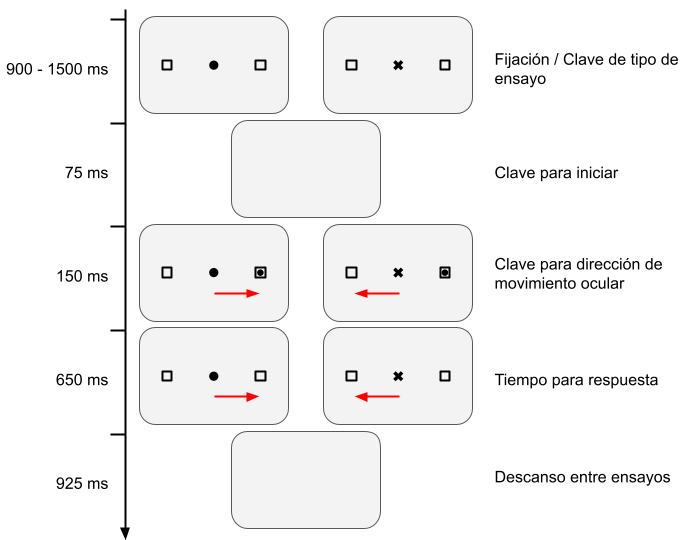
\includegraphics[width=0.8\linewidth]{media/antisaccades-protocol.png}}
    \caption{Protocolo de la tarea de antisacadas}
    \label{fig:antisaccades-protocol}
\end{figure}

\subsection{Preprocesamiento} \label{section:preprocessing}

En ambas instancias de experimentación el objetivo principal fue detectar
dirección y latencia de la respuesta dada por los sujetos.
Para lograr esto tuvieron que implementarse mecanismos que detectaran sacadas
en base a las estimaciones arrojadas por nuestro prototipo.
Sin embargo, dada la naturaleza remota de nuestra experimentación se obtuvieron
tanto frecuencia de muestreo distintas (Figura
\ref{fig:sampling-frequency-distribution}) como resoluciones de pantalla
distintas (Figura \ref{fig:widths-distribution}).
Para simplificar la implementación de la detección de sacadas se buscó
uniformizar los datos obtenidos de distintas fuentes a un mismo formato, además
se descartaron aquellos datos que se consideraron inválidos.
En ambas instancias se ignoraron los valores “y” de las estimaciones, pues para
nuestro caso de uso sólo interesaba capturar los movimientos horizontales de la
mirada.

\begin{figure}
  \centering
  TODO: load image
  \caption{Distribución de frecuencias de muestreo}
  \label{fig:sampling-frequency-distribution}
\end{figure}

\begin{figure}
  \centering
  TODO: load image
  \caption{Distribución de anchos de resoluciones}
  \label{fig:widths-distribution}
\end{figure}

En primer lugar, se descartaron las repeticiones cuyas estimaciones tuvieran
una frecuencia menor a 15 Hz.
Luego, a frecuencia de muestreo se uniformizó a 30 Hz realizando interpolación
lineal.
A partir del timestamp de la primera muestra se tomaron timestamps subsecuentes
cada 1000 / 30 ms.
Para cada uno de estos timestamps se interpoló la estimación correspondiente
utilizando la estimación anterior y la estimación posterior. 

% TODO: Rever cómo se explican las normalizaciones
%       capaz convenga hacer algun diagrama
Las estimaciones de la mirada fueron luego llevadas del rango variable por
sujeto al rango [-1, 1] buscando que al valor 0 fueran a caer las estimaciones
correspondientes a cuando el sujeto miraba al centro de la pantalla.
En la primera, instancia se normalizó cada tarea individualmente utilizando el
centro estimado de cada sujeto c (calculado como el promedio de los valores de
tal sujeto) y los valores mínimos $min_x$ y máximos $max_x$ de la repetición:
las estimaciones en el rango [$min_x$, c] se llevaron con interpolación lineal
al rango [-1, 0] y análogamente las estimaciones en el rango [c, $max_x$] se
llevaron al rango [0, 1].
Para la segunda instancia, la normalización se realizó en base a las
validaciones realizadas durante la tarea.
Para cada conjunto de repeticiones posteriores a una calibración + validación
se calcularon los valores l, c y r como el promedio de las estimaciones
obtenidas al mostrar respectivamente los estímulos de validación a izquierda,
centro y derecha.
Luego, similar a la instancia anterior, el rango [l, c] fue llevado al rango
[-1, 0] y el rango [c, r] fue llevado al rango [0, 1].

Post normalización, las estimaciones fueron modificadas tal que pudiera
asumirse que el estímulo lateral aparecía siempre del mismo lado.
Para esto, en las repeticiones en las cuales el estímulo visual aparecía a la
izquierda, se multiplicaron los valores de las estimaciones horizontales por
-1.
De esta manera se podrá asumir que si los valores de las estimaciones son
positivos entonces el sujeto miró al estímulo, mientras que si las estimaciones
son negativas entonces el sujeto habrá mirado en la dirección contraria.
Así, para identificar prosacadas correctas tendrá que verificarse que haya un
salto de valores cercanos a 0 a valores cercanos a 1, y análogamente para
identificar antisacadas correctas tendrá que verificarse un salto de valores
cercanos a 0 a valores cercanos a -1.

Se descartaron luego las repeticiones en las cuales el sujeto no estuviera
fijando la posición del estímulo de fijación durante los 500 ms previos a la
aparición del estímulo visual lateral.
Si un sujeto terminó con menos de 30 de repeticiones por tarea entonces se
descartó también el resto de sus repeticiones.
Además se descartaron a mano las repeticiones de sujetos cuyos datos se
considerarán inválidos.
